\documentclass{beamer}

\usepackage[T1,T2A]{fontenc}
\usepackage[utf8]{inputenc}
\usepackage[english,russian]{babel}
\usepackage{hyperref}
\usepackage{microtype}
\usepackage{csquotes}
\usepackage{amsmath}
\usepackage{amsthm}
\usepackage{amssymb}
\usepackage{mathtext}
\usepackage{physics}
\usepackage{newfloat}
\usepackage{caption}
\usepackage{indentfirst}
\usepackage{hyperref}
\usepackage{mdframed}
\usepackage{graphicx}
\usepackage{subfig}
\usepackage{appendix}

%% workaround for the \@ifundefined macro update in the 2018 LaTeX release
%% should be fixed in one of the next releases of caption.sty
\makeatletter
\let\@@magyar@captionfix\relax
\makeatother

\DeclareGraphicsExtensions{.pdf,.png,.jpg,.PNG}
\graphicspath{{./img/}}
\captionsetup[figure]{justification=centering}
\renewcommand{\thesubfigure}{\asbuk{subfigure}}
\DeclareCaptionLabelSeparator{dotseparator}{. }
\captionsetup{labelsep=dotseparator}
\makeatletter\appto{\appendices}{\def\Hy@chapapp{Appendix}}\makeatother
\renewcommand{\appendixtocname}{Приложения}
\renewcommand{\appendixpagename}{Приложения}
\setbeamertemplate{background canvas}[vertical shading][bottom=red!2,top=green!2]

\usetheme{Ilmenau}
\usecolortheme{spruce}
\usefonttheme[onlysmall]{serif}

\setbeamercolor{title in head/foot}{parent=palette primary}
\setbeamercolor{author in head/foot}{parent=palette primary}
\setbeamercolor{institute in head/foot}{parent=palette primary}

\setbeamercolor{title}{fg=black}
\setbeamercolor{frametitle}{fg=black}
\setbeamercolor*{enumerate item}{fg=black}

\setbeamercolor*{bibliography item}{fg=black}
\setbeamercolor*{bibliography entry title}{fg=black}
\setbeamercolor*{bibliography entry author}{fg=black}
\setbeamercolor*{bibliography entry location}{fg=black}
\setbeamercolor*{bibliography entry note}{fg=black}

\setbeamertemplate{enumerate item}[default]
\setbeamertemplate{bibliography entry title}{}
\setbeamertemplate{bibliography entry location}{}
\setbeamertemplate{bibliography entry note}{}
\setbeamertemplate{bibliography item}{\insertbiblabel}

\addtobeamertemplate{navigation symbols}{}{%
    \usebeamerfont{footline}%
    \usebeamercolor[fg]{title}%
    \hspace{1em}%
    \insertframenumber/\inserttotalframenumber
}

\hypersetup{
    colorlinks,
    citecolor=black,
    filecolor=black,
    linkcolor=black,
    urlcolor=black
}

\AtBeginSection[]{
  \begin{frame}
  \vfill
  \centering
  \begin{beamercolorbox}[sep=8pt,center,shadow=true,rounded=true]{title}
    \usebeamerfont{title}\insertsection\par%
  \end{beamercolorbox}
  \vfill
  \end{frame}
}

\DeclareMathOperator{\Rot}{\mathbf{rot}}
\DeclareMathOperator{\Grad}{\mathbf{grad}}
\DeclareMathOperator{\Div}{\mathbf{div}}
\DeclareMathOperator{\D}{D}
\newcommand{\V}[1]{\mathbf{#1}}
\newcommand{\Op}[1]{\hat{\V{#1}}}


\deftranslation[to=russian]{Theorem}{Теорема}
\deftranslation[to=russian]{theorem}{Теорема}

\title{Тепловое излучение\\ в сферическом резонаторе}
\author[Василевский~А.В.]{
    Василевский~А.В. \\[\baselineskip]
    {\footnotesize Научный руководитель: Бурланков~Д.Е.}
}
\institute[ННГУ]{Нижегородский университет им. Н.И.~Лобачевского}
\date{2017}

\begin{document}

    %
    %
    %
    %%%%%%%%%%%%%%%%%%%%%%%%%%%%%%%%%%%%%%%%%%%%%%%%%%%%%%%%%%%%%%%%%%%%%%%
    %                            FRAME                                    %
    %%%%%%%%%%%%%%%%%%%%%%%%%%%%%%%%%%%%%%%%%%%%%%%%%%%%%%%%%%%%%%%%%%%%%%%
    %
    %
    %

    \frame{\titlepage}

    %
    %
    %
    %%%%%%%%%%%%%%%%%%%%%%%%%%%%%%%%%%%%%%%%%%%%%%%%%%%%%%%%%%%%%%%%%%%%%%%
    %                            FRAME                                    %
    %%%%%%%%%%%%%%%%%%%%%%%%%%%%%%%%%%%%%%%%%%%%%%%%%%%%%%%%%%%%%%%%%%%%%%%
    %
    %
    %

    \begin{frame}\frametitle{Введение}

        \begin{itemize}

            \item Резонаторы в современной науке имеют важнейшее значение. Одним из ключевых направлений развития физики сегодня является квантовая теория измерений и связанный с ней интерес к манипуляциям с отдельными квантовыми объектами.

            \item В связи с обнаружением сверхузких резонансов рассеяния и возможностью создания на этой основе микрорезонаторов с гигантской добротностью, интерес к этому вопросу усилился многократно.

            \item Анализ путей диссипации энергии в микрорезонаторах является задачей, требующей особого внимания.

        \end{itemize}

    \end{frame}

    %
    %
    %
    %%%%%%%%%%%%%%%%%%%%%%%%%%%%%%%%%%%%%%%%%%%%%%%%%%%%%%%%%%%%%%%%%%%%%%%
    %                            FRAME                                    %
    %%%%%%%%%%%%%%%%%%%%%%%%%%%%%%%%%%%%%%%%%%%%%%%%%%%%%%%%%%%%%%%%%%%%%%%
    %
    %
    %

    \begin{frame}\frametitle{Оптический микрорезонатор МШГ}

        \begin{figure}[h]
            \centering
            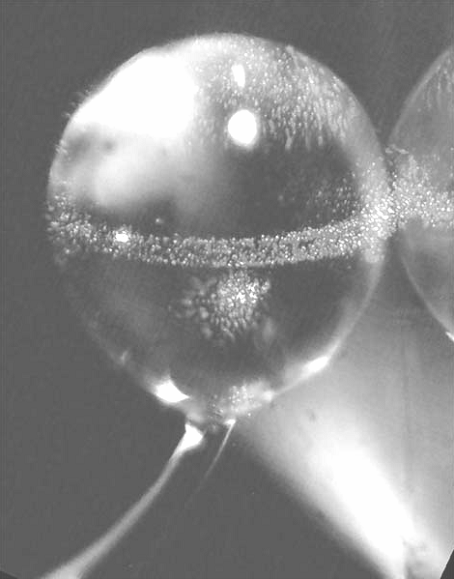
\includegraphics[width=\textwidth,height=0.6\textheight,keepaspectratio]{spherical_resonator}
            \caption[]{Оптический сферический микрорезонатор на ножке рядом с возбуждающей призмой, в которой видно его отражение. Диаметр около $570$ мкм, добротность $> 10^9$. Физический факультет МГУ \cite{microresonators}}
            \label{fig:spherical_resonator}
        \end{figure}

    \end{frame}

    %
    %
    %
    %%%%%%%%%%%%%%%%%%%%%%%%%%%%%%%%%%%%%%%%%%%%%%%%%%%%%%%%%%%%%%%%%%%%%%%
    %                            FRAME                                    %
    %%%%%%%%%%%%%%%%%%%%%%%%%%%%%%%%%%%%%%%%%%%%%%%%%%%%%%%%%%%%%%%%%%%%%%%
    %
    %
    %

    \begin{frame}\frametitle{Постановка задачи}

        \textbf{Цель работы}~--- построение мод электромагнитного поля в сферическом резонаторе и исследование их термодинамики.

        \begin{itemize}

            \item В работе применен подход, в основе которого лежат векторы Киллинга объемлющего пространства.

            \item Методика применена к скалярным и векторным полям (электромагнитному полю).

            \item Планируется исследование термодинамических характеристик излучения в сферическом резонаторе на основе полученных мод электромагнитного поля.

        \end{itemize}

    \end{frame}

    %
    %
    %
    %%%%%%%%%%%%%%%%%%%%%%%%%%%%%%%%%%%%%%%%%%%%%%%%%%%%%%%%%%%%%%%%%%%%%%%
    %                            FRAME                                    %
    %%%%%%%%%%%%%%%%%%%%%%%%%%%%%%%%%%%%%%%%%%%%%%%%%%%%%%%%%%%%%%%%%%%%%%%
    %
    %
    %

    \begin{frame}\frametitle{Уравнение на сферические моды}

        \begin{itemize}

            \item Уравнение на сферические моды~--- волновое уравнение для вектора напряженности $\V{E}$:
            %
            \begin{equation}\label{eq:wave_equation}
                \Delta \V{E} = - \lambda \V{E} ; \quad
                    \lambda = \varepsilon \frac{\omega^2}{c^2} .
            \end{equation}

            \item \autoref{eq:wave_equation}~--- уравнение на собственные функции и собственные значения (моды) оператора Лапласа $\Delta$.

            \item В задаче о сферическом резонаторе спектр мод дискретен и определяется тремя числами, $l$, $m$ и $n$.

        \end{itemize}

    \end{frame}

    %
    %
    %
    %%%%%%%%%%%%%%%%%%%%%%%%%%%%%%%%%%%%%%%%%%%%%%%%%%%%%%%%%%%%%%%%%%%%%%%
    %                            FRAME                                    %
    %%%%%%%%%%%%%%%%%%%%%%%%%%%%%%%%%%%%%%%%%%%%%%%%%%%%%%%%%%%%%%%%%%%%%%%
    %
    %
    %

    \begin{frame}\frametitle{Решение волнового уравнения}

        \begin{itemize}

            \item Сопряжено со значительными трудностями.

            \item Классические подходы громоздки и не обобщаются на поля произвольной тензорной размерности \cite{burlankov_tmf}.

            \item Операторный вид уравнения позволяет эффективно применить теорию операторов.

            \item Подход, основанный на операторах Киллинга, коммутирующих с оператором Лапласа, может быть обобщен на произвольные пространства и поля \cite{burlankov_tmf}.

        \end{itemize}

    \end{frame}

    %
    %
    %
    %%%%%%%%%%%%%%%%%%%%%%%%%%%%%%%%%%%%%%%%%%%%%%%%%%%%%%%%%%%%%%%%%%%%%%%
    %                            FRAME                                    %
    %%%%%%%%%%%%%%%%%%%%%%%%%%%%%%%%%%%%%%%%%%%%%%%%%%%%%%%%%%%%%%%%%%%%%%%
    %
    %
    %

    \begin{frame}\frametitle{Операторы Киллинга}

        \begin{itemize}

            \item Ли-вариация $\delta_\xi\tau$ ~--- инвариантное обобщение производной по направлению на произвольные тензорные поля \cite{lie_derivative_theory,symmetry_and_killing_fields}. В координатном представлении
            %
            \begin{equation}\begin{aligned}
                \delta_\xi {T^{a_1 \dots a_p}}_{b_1 \dots b_q}
                    &= \xi^c \left( \partial_c {T^{a_i \dots a_p}}_{b_1 \dots b_q} \right) \\
                    &- \left( \partial_{c} \xi^{a_1} \right) {T^{c a_2 \dots a_p}}_{b_1 \dots b_q} - \dots \\
                    &+ \left( \partial_{b_1} \xi^c \right) {T^{a_1 \dots a_p}}_{c b_2 \dots b_q} + \dots .
            \end{aligned}\end{equation}

            \item Метрический тензор $g_{ij}$ полностью определяет метрику риманова пространства.

            \item Векторные поля, на которых Ли-вариация метрического тензора равна нулю, называются движениями, или полями Киллинга.

        \end{itemize}

    \end{frame}

    %
    %
    %
    %%%%%%%%%%%%%%%%%%%%%%%%%%%%%%%%%%%%%%%%%%%%%%%%%%%%%%%%%%%%%%%%%%%%%%%
    %                            FRAME                                    %
    %%%%%%%%%%%%%%%%%%%%%%%%%%%%%%%%%%%%%%%%%%%%%%%%%%%%%%%%%%%%%%%%%%%%%%%
    %
    %
    %

    \begin{frame}\frametitle{Операторы Киллинга и поля Киллинга}

        Коммутатор векторных полей вводится посредством Ли-вариации:
        %
        \begin{equation}\begin{aligned}\label{eq:vector_field_commutator}
            \delta_\xi T^a
                = \xi^c \partial_c T^a - T^c \partial_{c} \xi^a
                \equiv [\xi, T]^a.
        \end{aligned}\end{equation}

        \begin{theorem}[О коммутации]
            Операторы Киллинга коммутируют, если коммутирую порождающие их поля.
        \end{theorem}

    \end{frame}

    %
    %
    %
    %%%%%%%%%%%%%%%%%%%%%%%%%%%%%%%%%%%%%%%%%%%%%%%%%%%%%%%%%%%%%%%%%%%%%%%
    %                            FRAME                                    %
    %%%%%%%%%%%%%%%%%%%%%%%%%%%%%%%%%%%%%%%%%%%%%%%%%%%%%%%%%%%%%%%%%%%%%%%
    %
    %
    %

    \begin{frame}\frametitle{Поля Киллинга евклидова пространства}

        В трехмерном евклидовом пространстве существует шесть полей Киллинга. В декартовых координатах:
        %
        \begin{equation}
            \V{\xi}_i
            =
            \left[
                \V{n}_x, \V{n}_y, \V{n}_z,
                \V{l}_x, \V{l}_y, \V{l}_z
            \right]
            =
            \begin{bmatrix}
                1 & 0 & 0 & 0  & -z & y  \\
                0 & 1 & 0 & z  & 0  & -x \\
                0 & 0 & 1 & -y & x  & 0
            \end{bmatrix}
        \end{equation}

        Первая тройка образует группу движений трансляций, вторая~--- группу движений вращений.

    \end{frame}

    %
    %
    %
    %%%%%%%%%%%%%%%%%%%%%%%%%%%%%%%%%%%%%%%%%%%%%%%%%%%%%%%%%%%%%%%%%%%%%%%
    %                            FRAME                                    %
    %%%%%%%%%%%%%%%%%%%%%%%%%%%%%%%%%%%%%%%%%%%%%%%%%%%%%%%%%%%%%%%%%%%%%%%
    %
    %
    %

    \begin{frame}\frametitle{Поля Киллинга в сферических координатах}

        Переведем поля Киллинга в сферическую систему координат. В контравариантных компонентах получим:
        %
        \begin{equation}
            \V{n}_i
            =
            \begin{bmatrix}
                \sin\theta \cos\varphi          & \sin\theta \sin\varphi        & \cos\theta \\
                r^{-1} \cos\theta \cos\varphi   & r^{-1} \cos\theta \sin\varphi & - r^{-1} \sin\theta \\
                - r^{-1} \csc\theta \sin\varphi & r^{-1} \csc\theta \cos\varphi & 0
            \end{bmatrix}
            ,
        \end{equation}
        %
        \begin{equation}
            \V{l}_i
            =
            \begin{bmatrix}
                0
                    & 0
                    & 0 \\
                \sin\varphi
                    & \cos\varphi
                    & 0 \\
                \cos\varphi \cot\theta
                    & \cot\theta \sin\varphi
                    & - 1
            \end{bmatrix}
            .
        \end{equation}

        Наибольшее значение для нас будет иметь группа движений вращений. Следует отметить уже сейчас, что $\V{l}_z$ не зависит ни от одной из координат пространства.

    \end{frame}

    %
    %
    %
    %%%%%%%%%%%%%%%%%%%%%%%%%%%%%%%%%%%%%%%%%%%%%%%%%%%%%%%%%%%%%%%%%%%%%%%
    %                            FRAME                                    %
    %%%%%%%%%%%%%%%%%%%%%%%%%%%%%%%%%%%%%%%%%%%%%%%%%%%%%%%%%%%%%%%%%%%%%%%
    %
    %
    %

    \begin{frame}\frametitle{Коммутационные соотношения операторов Киллинга}

        Коммутационные соотношения внутри и между группами движений евклидова пространства:
        %
        \begin{equation}
            \begin{bmatrix}
                [ \Op{n}_x \Op{n}_y ] & [ \Op{n}_z \Op{n}_x ] & [ \Op{n}_y \Op{n}_z ] \\
                [ \Op{l}_x \Op{l}_y ] & [ \Op{l}_z \Op{l}_x ] & [ \Op{l}_y \Op{l}_z ] \\
                [ \Op{n}_x \Op{l}_x ] & [ \Op{n}_y \Op{l}_x ] & [ \Op{n}_z \Op{l}_x ] \\
                [ \Op{n}_x \Op{l}_y ] & [ \Op{n}_y \Op{l}_y ] & [ \Op{n}_z \Op{l}_y ] \\
                [ \Op{n}_x \Op{l}_z ] & [ \Op{n}_y \Op{l}_z ] & [ \Op{n}_z \Op{l}_z ]
            \end{bmatrix}
            =
            \begin{bmatrix}
                0          &   0        &   0        \\
                \Op{l}_z   &   \Op{l}_y &   \Op{l}_x \\
                0          &   \Op{n}_z & - \Op{n}_y \\
                - \Op{n}_z &   0        &   \Op{n}_x \\
                \Op{n}_y   & - \Op{n}_x &   0
            \end{bmatrix}
        \end{equation}

        Оператор Лапласа в декартовых координатах:
        %
        \begin{equation}
            \Delta = \Op{n}_x\Op{n}_x + \Op{n}_y\Op{n}_y + \Op{n}_z\Op{n}_z .
        \end{equation}
        %
        Операторы Киллинга коммутируют с оператором Лапласа.

    \end{frame}

    %
    %
    %
    %%%%%%%%%%%%%%%%%%%%%%%%%%%%%%%%%%%%%%%%%%%%%%%%%%%%%%%%%%%%%%%%%%%%%%%
    %                            FRAME                                    %
    %%%%%%%%%%%%%%%%%%%%%%%%%%%%%%%%%%%%%%%%%%%%%%%%%%%%%%%%%%%%%%%%%%%%%%%
    %
    %
    %

    \begin{frame}\frametitle{Производные операторы Киллинга}

        \begin{enumerate}
            \item Операторы вращений не коммутируют.

            \item Составим оператор $\Op{l}^2 = \Op{l}_x \Op{l}_x + \Op{l}_y \Op{l}_y + \Op{l}_z \Op{l}_z$. Он коммутирует со всеми операторами вращений.

            \item Введем операторы повышения и понижения, $\Op{l}_{+} = \Op{l}_x - i\Op{l}_y$ и $\Op{l}_{-} = \Op{l}_x + i\Op{l}_y$. Коммутационные соотношения:
            %
            \begin{equation}
                \left[ \Op{l}_{+}, \Op{l}_{-} \right] = 2 i \Op{l}_{z} ; \quad
                \left[ \Op{l}_{z}, \Op{l}_{+} \right] =   i \Op{l}_{+} ; \quad
                \left[ \Op{l}_{z}, \Op{l}_{-} \right] = - i \Op{l}_{-} .
            \end{equation}
            %
            Операторы повышения и понижения коммутируют с $\Op{l}^2$.
        \end{enumerate}

    \end{frame}

    %
    %
    %
    %%%%%%%%%%%%%%%%%%%%%%%%%%%%%%%%%%%%%%%%%%%%%%%%%%%%%%%%%%%%%%%%%%%%%%%
    %                            FRAME                                    %
    %%%%%%%%%%%%%%%%%%%%%%%%%%%%%%%%%%%%%%%%%%%%%%%%%%%%%%%%%%%%%%%%%%%%%%%
    %
    %
    %

    \begin{frame}\frametitle{Собственные моды операторов Киллинга}

        Пусть
        %
        \begin{equation}\begin{gathered}
            \Op{l}^2 h_{\lambda,m} = \lambda h_{\lambda,m} ; \quad
            \Op{l}_z h_{\lambda,m} = i m h_{\lambda,m} .
        \end{gathered}\end{equation}

        Можно показать, что
        %
        \begin{equation}\begin{gathered}
            \Op{l}_z \Op{l}_{+} h_{\lambda,m} = i (m + 1) h_{\lambda,m+1} \\
            \Op{l}_z \Op{l}_{-} h_{\lambda,m} = i (m - 1) h_{\lambda,m-1} ,
        \end{gathered}\end{equation}
        %
        и что
        %
        \begin{equation}\begin{gathered}
            \Op{l}_z \Op{l}_{+} h_{\lambda,l} = 0 ; \quad
            \Op{l}_z \Op{l}_{-} h_{\lambda,-l} = 0 .
        \end{gathered}\end{equation}

        В итоге $\lambda = l (l + 1)$, $- l \le m \le l$.

    \end{frame}

    %
    %
    %
    %%%%%%%%%%%%%%%%%%%%%%%%%%%%%%%%%%%%%%%%%%%%%%%%%%%%%%%%%%%%%%%%%%%%%%%
    %                            FRAME                                    %
    %%%%%%%%%%%%%%%%%%%%%%%%%%%%%%%%%%%%%%%%%%%%%%%%%%%%%%%%%%%%%%%%%%%%%%%
    %
    %
    %

    \begin{frame}\frametitle{Базовые моды}

        Наиболее интересной является базовая мода, т.е. мода с $m = 0$, для которой
        %
        \begin{equation}
            \Op{l}_z h_{l, 0} = 0 .
        \end{equation}

        Подействуем на нее оператором $\Op{l}_z$:
        %
        \begin{equation}
            \Op{l}_z h_{l, 0} = \pdv{h_{l, 0}}{\varphi} = 0 .
        \end{equation}
        %
        Базовая мода не зависит от $\varphi$. Кроме того, базовая мода удовлетворяет соотношению:
        %
        \begin{equation}\label{eq:basemode_eq}
            \Op{l}^2 h_{l, 0}
                = \qty( \Op{l}_{+} \Op{l}_{-} + \Op{l}_z^2 - i \Op{l}_z ) h_{l, 0}
                = \Op{l}_{+} \Op{l}_{-} h_{l, 0}
                = - l (l + 1) h_{l, 0} .
        \end{equation}

    \end{frame}

    %
    %
    %
    %%%%%%%%%%%%%%%%%%%%%%%%%%%%%%%%%%%%%%%%%%%%%%%%%%%%%%%%%%%%%%%%%%%%%%%
    %                            FRAME                                    %
    %%%%%%%%%%%%%%%%%%%%%%%%%%%%%%%%%%%%%%%%%%%%%%%%%%%%%%%%%%%%%%%%%%%%%%%
    %
    %
    %

    \begin{frame}\frametitle{Методика нахождения сферических мод}

        \begin{enumerate}
            \item Построение базовых мод с $m = 0$ и определенным $l$;
            \item Нахождение радиальных функций для базовых мод;
            \item Получение остальных $2l$ производных мод с $m = \pm 1, \pm 2, \dots$ путем применения операторов повышения и понижения.
        \end{enumerate}

    \end{frame}

    %
    %
    %
    %%%%%%%%%%%%%%%%%%%%%%%%%%%%%%%%%%%%%%%%%%%%%%%%%%%%%%%%%%%%%%%%%%%%%%%
    %                            FRAME                                    %
    %%%%%%%%%%%%%%%%%%%%%%%%%%%%%%%%%%%%%%%%%%%%%%%%%%%%%%%%%%%%%%%%%%%%%%%
    %
    %
    %

    \begin{frame}\frametitle{Скалярные моды}

        В скалярном случае операторы Киллинга~--- просто дифференциальные операторы первого порядка:
        %
        \begin{equation}
            \Op{\xi} = \xi^i \pdv*{x^i} .
        \end{equation}
        %
        Выпишем основные необходимые нам операторы Киллинга:
        %
        \begin{equation}\begin{gathered}
            \Op{l}_{+} f = \exp(i\varphi) \qty(\cot(\theta) f'_\varphi - i f'_\theta) \\
            \Op{l}_{-} f = \exp(-i\varphi) \qty(\cot(\theta) f'_\varphi + i f'_\theta) \\
            \Op{l}_z f   = f'_\varphi .
        \end{gathered}\end{equation}

        Моду $h_{l,m}$ представим в виде произведения:
        %
        \begin{equation}
            h_{l,m}(r,\theta,\varphi) = f(r) f_{l,m}(\theta,\varphi) .
        \end{equation}

        Базовая мода тогда запишется в виде:
        %
        \begin{equation}
            h_{l,0}(r,\theta) = f(r) f_{l,0}(\theta) .
        \end{equation}

    \end{frame}

    %
    %
    %
    %%%%%%%%%%%%%%%%%%%%%%%%%%%%%%%%%%%%%%%%%%%%%%%%%%%%%%%%%%%%%%%%%%%%%%%
    %                            FRAME                                    %
    %%%%%%%%%%%%%%%%%%%%%%%%%%%%%%%%%%%%%%%%%%%%%%%%%%%%%%%%%%%%%%%%%%%%%%%
    %
    %
    %

    \begin{frame}\frametitle{Скалярные угловые моды~--- получение}

        Уравнение (\autoref{eq:basemode_eq}) на угловую часть базовой моды $f_{l,0}(\theta) \equiv f_l(\theta)$:
        %
        \begin{equation}
            \Op{l}_{+} \Op{l}_{-} f_l + l (l + 1) f_l = 0 .
        \end{equation}
        %
        Раскроем операторы повышения и понижения. Получим дифференциальное уравнение второго порядка:
        %
        \begin{equation}
            f_l''(\theta) + f_l'(\theta) \cot \theta + l (l + 1) f_l(\theta) = 0 .
        \end{equation}
        %
        Данное уравнение определяет $P$- и $Q$-полиномы Лежандра. $Q$-полиномы не регулярны в нуле. Отсюда
        %
        \begin{equation}\label{eq:basemode_angle}
            f_{l,0} = P_l(\cos\theta) .
        \end{equation}

    \end{frame}

    %
    %
    %
    %%%%%%%%%%%%%%%%%%%%%%%%%%%%%%%%%%%%%%%%%%%%%%%%%%%%%%%%%%%%%%%%%%%%%%%
    %                            FRAME                                    %
    %%%%%%%%%%%%%%%%%%%%%%%%%%%%%%%%%%%%%%%%%%%%%%%%%%%%%%%%%%%%%%%%%%%%%%%
    %
    %
    %

    \begin{frame}

        Получим угловые части производных мод ($m \neq 0$). Применим к \autoref{eq:basemode_angle} оператор повышения $m$ раз:
        %
        \begin{center}
            \begin{tabular}{|c|c|c|}\hline
                $m$ & \multicolumn{2}{|c|}{$f_{l,m}$} \\ \hline
                $1$ & $i \exp(i\varphi) \sin(\theta) {P_l}'(\cos\theta)$
                    & $- i \exp(i\varphi) P^1_l(\cos\theta)$ \\ \hline
                $2$ & $- \exp(2i\varphi) \sin^2(\theta) {P_l}''(\cos\theta)$
                    & $- \exp(2i\varphi) P^2_l(\cos\theta)$ \\ \hline
                $3$ & $- i \exp(3i\varphi) \sin^3(\theta) {P_l}'''(\cos\theta)$
                    & $i \exp(3i\varphi) P^3_l(\cos\theta)$ \\ \hline
                $4$ & $\exp(4i\varphi) \sin^4(\theta) {P_l}''''(\cos\theta)$
                    & $\exp(4i\varphi) P^4_l(\cos\theta)$ \\ \hline
                $5$ & $i \exp(5i\varphi) \sin^5(\theta) {P_l}'''''(\cos\theta)$
                    & $- i \exp(5i\varphi) P^5_l(\cos\theta)$ \\ \hline
            \end{tabular} ,
        \end{center}
        %
        \begin{equation}
            P^m_l(\cos\theta) = (-1)^m \sin^m \theta \dv[m]{P_l\qty(\cos\theta)}{\qty(\cos\theta)} .
        \end{equation}

        Из приведенной таблицы заключаем, что общий вид производной моды следующий:
        %
        \begin{equation}
            f_{l,m}(\theta,\varphi)
                = \Op{l}^m_{+} f_l(\theta)
                = (-i)^m \exp(i m \varphi) P^m_l\qty(\cos\theta) .
        \end{equation}

    \end{frame}

    %
    %
    %
    %%%%%%%%%%%%%%%%%%%%%%%%%%%%%%%%%%%%%%%%%%%%%%%%%%%%%%%%%%%%%%%%%%%%%%%
    %                            FRAME                                    %
    %%%%%%%%%%%%%%%%%%%%%%%%%%%%%%%%%%%%%%%%%%%%%%%%%%%%%%%%%%%%%%%%%%%%%%%
    %
    %
    %

    \begin{frame}\frametitle{Скалярные угловые моды}

        \begin{figure}[h]
            \centering
            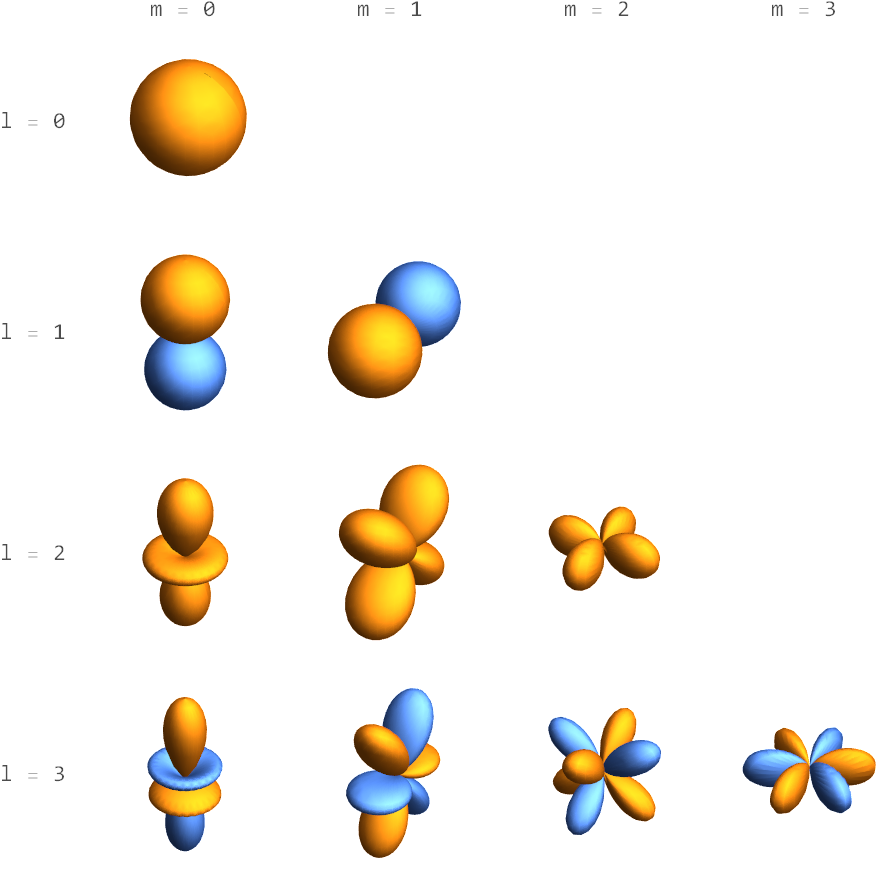
\includegraphics[width=\textwidth,height=0.6\textheight,keepaspectratio]{angle_modes}
            \caption[]{Скалярные угловые моды для нескольких $l$}
            \label{fig:angle_modes}
        \end{figure}

    \end{frame}

    %
    %
    %
    %%%%%%%%%%%%%%%%%%%%%%%%%%%%%%%%%%%%%%%%%%%%%%%%%%%%%%%%%%%%%%%%%%%%%%%
    %                            FRAME                                    %
    %%%%%%%%%%%%%%%%%%%%%%%%%%%%%%%%%%%%%%%%%%%%%%%%%%%%%%%%%%%%%%%%%%%%%%%
    %
    %
    %

    \begin{frame}\frametitle{Скалярные радиальные моды~--- получение}

        Найдем вид $f(r)$, при котором базовая мода $h_{l,0}(r,\theta) = f(r) f_{l,0}(\theta)$ является собственной для оператора Лапласа:
        %
        \begin{equation}\label{eq:basemode_lap}
            \Delta h_{l,0} = - \lambda h_{l,0} .
        \end{equation}
        %
        Оператор Лапласа коммутирует с операторами повышения и понижения, потому $f_{l,0}(\theta)$ уже является собственной функцией оператора Лапласа, а значит \autoref{eq:basemode_lap} должно удовлетворяться для любого $\theta$. Из этого следует дифференциальное уравнение на $f(r)$:
        %
        \begin{equation}
            r^2 f''(r) + 2 r f'(r) + (\lambda r^2 - l(l+1)) f(r) = 0 .
        \end{equation}

    \end{frame}

    %
    %
    %
    %%%%%%%%%%%%%%%%%%%%%%%%%%%%%%%%%%%%%%%%%%%%%%%%%%%%%%%%%%%%%%%%%%%%%%%
    %                            FRAME                                    %
    %%%%%%%%%%%%%%%%%%%%%%%%%%%%%%%%%%%%%%%%%%%%%%%%%%%%%%%%%%%%%%%%%%%%%%%
    %
    %
    %

    \begin{frame}

        Его решение~--- сферические $J$- и $Y$-функции Бесселя, получаемые из обычных по формулам:
        %
        \begin{equation}
            j_n(r) = \frac{\sqrt{\pi/2}}{\sqrt{r}} J_{n+\frac{1}{2}}(r) ; \quad
            y_n(r) = \frac{\sqrt{\pi/2}}{\sqrt{r}} Y_{n+\frac{1}{2}}(r) .
        \end{equation}
        %
        $Y$-функции не регулярны в нуле, потому не интересны.

        Итак,
        %
        \begin{equation}
            f(r) = j_l(\sqrt{\lambda} r) ,
        \end{equation}
        %
        \begin{equation}
            f_{l,m}(r,\theta,\varphi)
                = j_l(\sqrt{\lambda} r) (-i)^m \exp(i m \varphi) P^m_l\qty(\cos\theta) .
        \end{equation}

    \end{frame}

    %
    %
    %
    %%%%%%%%%%%%%%%%%%%%%%%%%%%%%%%%%%%%%%%%%%%%%%%%%%%%%%%%%%%%%%%%%%%%%%%
    %                            FRAME                                    %
    %%%%%%%%%%%%%%%%%%%%%%%%%%%%%%%%%%%%%%%%%%%%%%%%%%%%%%%%%%%%%%%%%%%%%%%
    %
    %
    %

    \begin{frame}\frametitle{Скалярные радиальные моды}

        \begin{figure}[h]
            \centering
            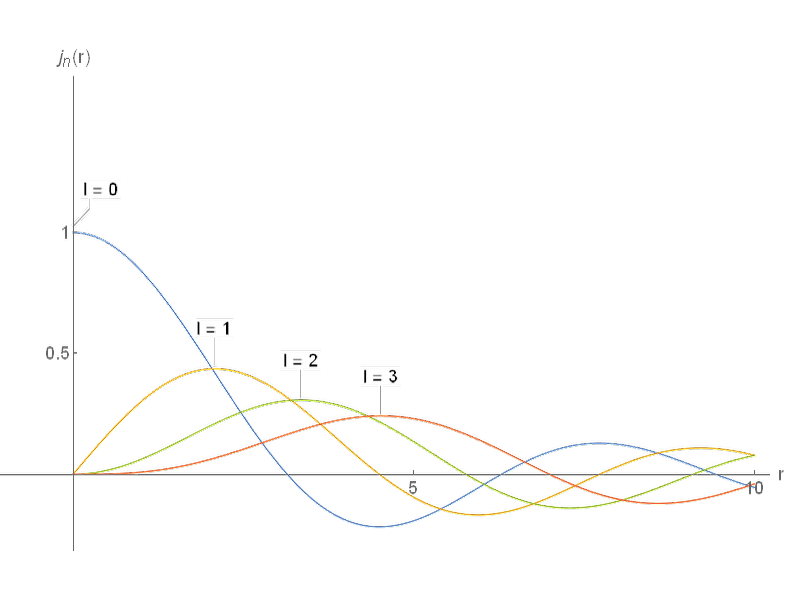
\includegraphics[width=\textwidth,height=0.6\textheight,keepaspectratio]{radial_modes}
            \caption[]{Скалярные радиальные моды для нескольких $l$}
            \label{fig:radial_modes}
        \end{figure}

    \end{frame}

    %
    %
    %
    %%%%%%%%%%%%%%%%%%%%%%%%%%%%%%%%%%%%%%%%%%%%%%%%%%%%%%%%%%%%%%%%%%%%%%%
    %                            FRAME                                    %
    %%%%%%%%%%%%%%%%%%%%%%%%%%%%%%%%%%%%%%%%%%%%%%%%%%%%%%%%%%%%%%%%%%%%%%%
    %
    %
    %

    \begin{frame}\frametitle{Векторные моды}

        Применительно к векторным полям операторы Киллинга~--- введенные ранее коммутаторы:
        %
        \begin{equation}\label{eq:killing_operator}
            \delta_\xi a^k
                = \xi^c \pdv{a^k}{x^c} - a^c \pdv{\xi^k}{x^c}
                \equiv [\xi, a]^k .
        \end{equation}

        Из-за наличия члена $a^c \pdv*{\xi^k}{x^c}$, пропорционального компонентам самого векторного поля, компоненты проварьированного на $\xi$ векторного поля $\vb{a}$ приобретают весьма сложный вид, что доставляет определенные трудности для прямого решения задачи.

    \end{frame}

    %
    %
    %
    %%%%%%%%%%%%%%%%%%%%%%%%%%%%%%%%%%%%%%%%%%%%%%%%%%%%%%%%%%%%%%%%%%%%%%%
    %                            FRAME                                    %
    %%%%%%%%%%%%%%%%%%%%%%%%%%%%%%%%%%%%%%%%%%%%%%%%%%%%%%%%%%%%%%%%%%%%%%%
    %
    %
    %

    \begin{frame}

        \begin{equation}\begin{gathered}\label{eq:killing_operators_vect}
            \Op{l}_z a^k = \pdv{a^k}{\varphi} \\
            \Op{l}_{+} a^k = \exp(i\varphi) \begin{pmatrix}
                \cot(\theta) \pdv{a^1}{\varphi} - i \pdv{a^1}{\theta} \\
                \cot(\theta) \pdv{a^2}{\varphi} - i \pdv{a^2}{\theta} - a^3 \\
                \cot(\theta) \pdv{a^3}{\varphi} - i \pdv{a^3}{\theta}
                    - i \cot(\theta) a^3 + \csc^2(\theta) a^2
            \end{pmatrix}^k \\
            \Op{l}_{-} a^k = \exp(-i\varphi) \begin{pmatrix}
                \cot(\theta) \pdv{a^1}{\varphi} + i \pdv{a^1}{\theta} \\
                \cot(\theta) \pdv{a^2}{\varphi} + i \pdv{a^2}{\theta} - a^3 \\
                \cot(\theta) \pdv{a^3}{\varphi} + i \pdv{a^3}{\theta}
                    + i \cot(\theta) a^3 + \csc^2(\theta) a^2
            \end{pmatrix}^k
        \end{gathered}\end{equation}

    \end{frame}

    %
    %
    %
    %%%%%%%%%%%%%%%%%%%%%%%%%%%%%%%%%%%%%%%%%%%%%%%%%%%%%%%%%%%%%%%%%%%%%%%
    %                            FRAME                                    %
    %%%%%%%%%%%%%%%%%%%%%%%%%%%%%%%%%%%%%%%%%%%%%%%%%%%%%%%%%%%%%%%%%%%%%%%
    %
    %
    %

    \begin{frame}\frametitle{Поляризации векторных мод}

        Поиск векторных мод общего вида весьма сложен. Можно поступить иначе и показать, что возможны две поляризации векторного поля $a$, удовлетворяющие волновому уравнению:
        %
        \begin{equation}\begin{aligned}
            \vb{a}_{\mathrm{I}} &= \qty{ a^r, a^\theta, 0 } \\
            \vb{a}_{\mathrm{II}} &= \qty{ 0, 0, a^\varphi } .
        \end{aligned}\end{equation}

        Применительно к электромагнитному полю конфигурации $\vb{E} = \qty{ E^r, E^\theta, 0 }$ и $\vb{E} = \qty{ 0, 0, E^\varphi }$ называются соответственно $TH$ и $TE$.

    \end{frame}

    %
    %
    %
    %%%%%%%%%%%%%%%%%%%%%%%%%%%%%%%%%%%%%%%%%%%%%%%%%%%%%%%%%%%%%%%%%%%%%%%
    %                            FRAME                                    %
    %%%%%%%%%%%%%%%%%%%%%%%%%%%%%%%%%%%%%%%%%%%%%%%%%%%%%%%%%%%%%%%%%%%%%%%
    %
    %
    %

    \begin{frame}\frametitle{Векторные моды~--- получение}

        Получение векторных мод основывается на том же общем подходе, что и получение скалярных. Операторы Киллинга берутся в виде \autoref{eq:killing_operators_vect}. Следуя методике построения сферических мод для обеих поляризаций поля $\vb{a}$, строятся угловые и радиальные части сферических векторных мод. Опуская громоздкие и мало чем примечательные выкладки, приведем окончательный результат расчета угловых частей:
        %
        \begin{equation}
            \vb{a} = \begin{pmatrix}
                C_1 P_l(\cos\theta) \\
                C_2 P_l^1(\cos\theta) \\
                0
            \end{pmatrix} , \quad
            \vb{b} = \begin{pmatrix}
                0 \\
                0 \\
                i C_3 \csc(\theta) P_l^1(\cos\theta)
            \end{pmatrix} .
        \end{equation}

    \end{frame}

    %
    %
    %
    %%%%%%%%%%%%%%%%%%%%%%%%%%%%%%%%%%%%%%%%%%%%%%%%%%%%%%%%%%%%%%%%%%%%%%%
    %                            FRAME                                    %
    %%%%%%%%%%%%%%%%%%%%%%%%%%%%%%%%%%%%%%%%%%%%%%%%%%%%%%%%%%%%%%%%%%%%%%%
    %
    %
    %

    \begin{frame}\frametitle{Векторные угловые моды}

        \begin{figure}[h]
            \centering
            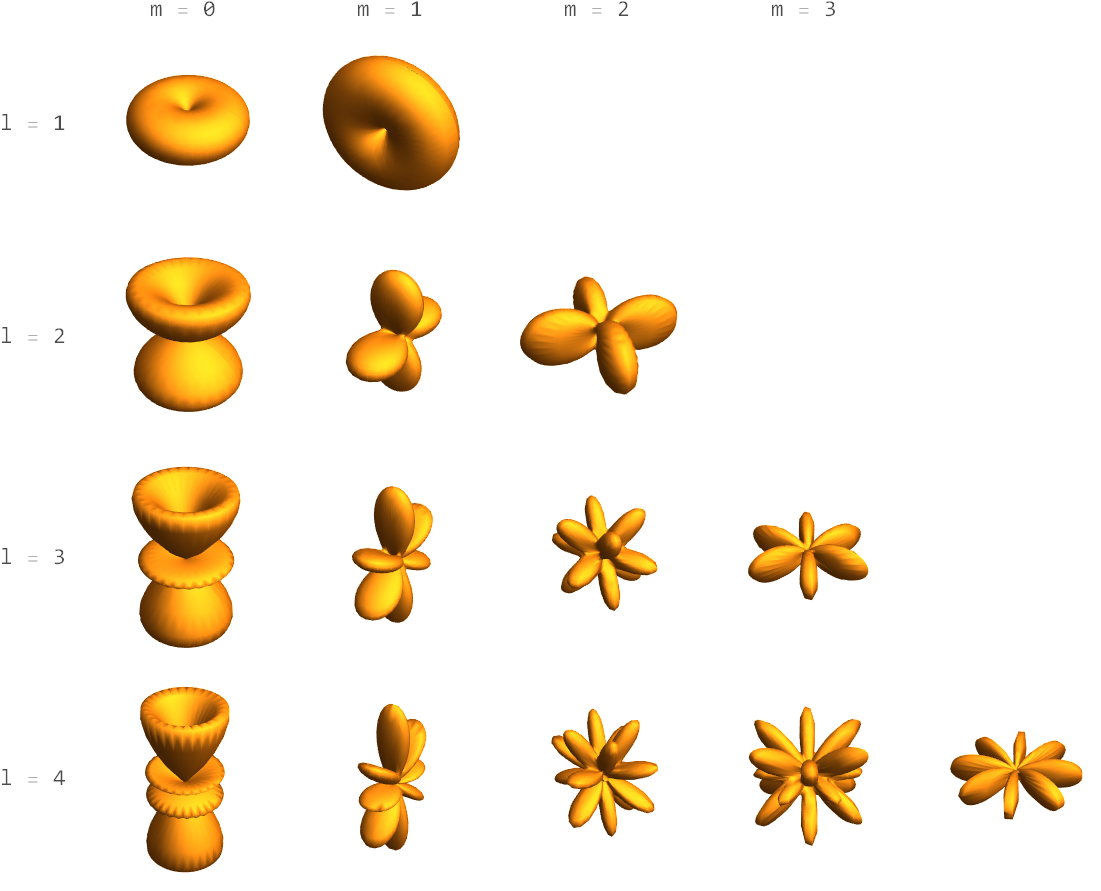
\includegraphics[width=\textwidth,height=0.6\textheight,keepaspectratio]{angle_modes_vect_ii}
            \caption[]{Векторные угловые моды для нескольких $l$ (изображена плотность энергии)}
            \label{fig:angle_modes_vect_ii}
        \end{figure}

    \end{frame}

    %
    %
    %
    %%%%%%%%%%%%%%%%%%%%%%%%%%%%%%%%%%%%%%%%%%%%%%%%%%%%%%%%%%%%%%%%%%%%%%%
    %                            FRAME                                    %
    %%%%%%%%%%%%%%%%%%%%%%%%%%%%%%%%%%%%%%%%%%%%%%%%%%%%%%%%%%%%%%%%%%%%%%%
    %
    %
    %

    \begin{frame}\frametitle{Выводы}

        \begin{itemize}
            \item В работе продемонстрировано применение методики Ли-генерации мод скалярного и векторного полей в трехмерном евклидовом пространстве.

            \item Получены угловые и радиальные части скалярных мод.

            \item Получены угловые части векторных мод.

            \item Математические выкладки проделаны для риманова пространства общего вида.
        \end{itemize}

    \end{frame}

    %
    %
    %
    %%%%%%%%%%%%%%%%%%%%%%%%%%%%%%%%%%%%%%%%%%%%%%%%%%%%%%%%%%%%%%%%%%%%%%%
    %                            FRAME                                    %
    %%%%%%%%%%%%%%%%%%%%%%%%%%%%%%%%%%%%%%%%%%%%%%%%%%%%%%%%%%%%%%%%%%%%%%%
    %
    %
    %

    \begin{frame}\frametitle{Заключение}

        Далее предстоит:
        %
        \begin{itemize}
            \item Получить радиальные части векторных мод.

            \item Применить граничные условия (пространство не пустое, а представляет собой сферический резонатор).

            \item Исследовать термодинамику резонатора.
        \end{itemize}

    \end{frame}

    %
    %
    %
    %%%%%%%%%%%%%%%%%%%%%%%%%%%%%%%%%%%%%%%%%%%%%%%%%%%%%%%%%%%%%%%%%%%%%%%
    %                        BIBLIOGRAPHY                                 %
    %%%%%%%%%%%%%%%%%%%%%%%%%%%%%%%%%%%%%%%%%%%%%%%%%%%%%%%%%%%%%%%%%%%%%%%
    %
    %
    %

    \begin{frame}\frametitle{Литература}
        \bibliographystyle{../../../lib/doc/bib/utf8gost705s}
        \bibliography{%
            ../../../lib/doc/bib/resonators,%
            ../../../lib/doc/bib/physics,%
            ../../../lib/doc/bib/math%
        }
    \end{frame}

\end{document}
